% Options for packages loaded elsewhere
\PassOptionsToPackage{unicode}{hyperref}
\PassOptionsToPackage{hyphens}{url}
%
\documentclass[
  ignorenonframetext,
]{beamer}
\usepackage{pgfpages}
\setbeamertemplate{caption}[numbered]
\setbeamertemplate{caption label separator}{: }
\setbeamercolor{caption name}{fg=normal text.fg}
\beamertemplatenavigationsymbolsempty
% Prevent slide breaks in the middle of a paragraph
\widowpenalties 1 10000
\raggedbottom
\setbeamertemplate{part page}{
  \centering
  \begin{beamercolorbox}[sep=16pt,center]{part title}
    \usebeamerfont{part title}\insertpart\par
  \end{beamercolorbox}
}
\setbeamertemplate{section page}{
  \centering
  \begin{beamercolorbox}[sep=12pt,center]{part title}
    \usebeamerfont{section title}\insertsection\par
  \end{beamercolorbox}
}
\setbeamertemplate{subsection page}{
  \centering
  \begin{beamercolorbox}[sep=8pt,center]{part title}
    \usebeamerfont{subsection title}\insertsubsection\par
  \end{beamercolorbox}
}
\AtBeginPart{
  \frame{\partpage}
}
\AtBeginSection{
  \ifbibliography
  \else
    \frame{\sectionpage}
  \fi
}
\AtBeginSubsection{
  \frame{\subsectionpage}
}
\usepackage{lmodern}
\usepackage{amssymb,amsmath}
\usepackage{ifxetex,ifluatex}
\ifnum 0\ifxetex 1\fi\ifluatex 1\fi=0 % if pdftex
  \usepackage[T1]{fontenc}
  \usepackage[utf8]{inputenc}
  \usepackage{textcomp} % provide euro and other symbols
\else % if luatex or xetex
  \usepackage{unicode-math}
  \defaultfontfeatures{Scale=MatchLowercase}
  \defaultfontfeatures[\rmfamily]{Ligatures=TeX,Scale=1}
\fi
\usetheme[]{default}
\usefonttheme{professionalfonts}
% Use upquote if available, for straight quotes in verbatim environments
\IfFileExists{upquote.sty}{\usepackage{upquote}}{}
\IfFileExists{microtype.sty}{% use microtype if available
  \usepackage[]{microtype}
  \UseMicrotypeSet[protrusion]{basicmath} % disable protrusion for tt fonts
}{}
\makeatletter
\@ifundefined{KOMAClassName}{% if non-KOMA class
  \IfFileExists{parskip.sty}{%
    \usepackage{parskip}
  }{% else
    \setlength{\parindent}{0pt}
    \setlength{\parskip}{6pt plus 2pt minus 1pt}}
}{% if KOMA class
  \KOMAoptions{parskip=half}}
\makeatother
\usepackage{xcolor}
\IfFileExists{xurl.sty}{\usepackage{xurl}}{} % add URL line breaks if available
\IfFileExists{bookmark.sty}{\usepackage{bookmark}}{\usepackage{hyperref}}
\hypersetup{
  pdftitle={Aleatorización por bloques},
  hidelinks,
  pdfcreator={LaTeX via pandoc}}
\urlstyle{same} % disable monospaced font for URLs
\newif\ifbibliography
\usepackage{graphicx}
\makeatletter
\def\maxwidth{\ifdim\Gin@nat@width>\linewidth\linewidth\else\Gin@nat@width\fi}
\def\maxheight{\ifdim\Gin@nat@height>\textheight\textheight\else\Gin@nat@height\fi}
\makeatother
% Scale images if necessary, so that they will not overflow the page
% margins by default, and it is still possible to overwrite the defaults
% using explicit options in \includegraphics[width, height, ...]{}
\setkeys{Gin}{width=\maxwidth,height=\maxheight,keepaspectratio}
% Set default figure placement to htbp
\makeatletter
\def\fps@figure{htbp}
\makeatother
\setlength{\emergencystretch}{3em} % prevent overfull lines
\providecommand{\tightlist}{%
  \setlength{\itemsep}{0pt}\setlength{\parskip}{0pt}}
\setcounter{secnumdepth}{-\maxdimen} % remove section numbering
\usepackage{fancyhdr}
\usepackage{lastpage}
\setbeamertemplate{navigation symbols}{}
\setbeamertemplate{footline}[page number]
\pagenumbering{arabic}
% \usepackage[mathbf,mathcal]{euler}
\usepackage{multicol}


\newenvironment{cols}[1][]{}{}

\newenvironment{col}[1]{\begin{minipage}{#1}\ignorespaces}{%
\end{minipage}
\ifhmode\unskip\fi
\aftergroup\useignorespacesandallpars}

\def\useignorespacesandallpars#1\ignorespaces\fi{%
#1\fi\ignorespacesandallpars}

\makeatletter
\def\ignorespacesandallpars{%
  \@ifnextchar\par
    {\expandafter\ignorespacesandallpars\@gobble}%
    {}%
}
\makeatother

\title{Aleatorización por bloques}
\author{Diseño e implementación de experimentos en ciencias sociales\\
\emph{Departamento de Economía (UdelaR)}}
\date{}

\begin{document}
\frame{\titlepage}

\begin{frame}{Análisis bajo asignación aleatoria por bloques}
\protect\hypertarget{anuxe1lisis-bajo-asignaciuxf3n-aleatoria-por-bloques}{}
\end{frame}

\hypertarget{experimentos-aleatorizados-por-bloque}{%
\section{Experimentos aleatorizados por
bloque}\label{experimentos-aleatorizados-por-bloque}}

\begin{frame}{Experimentos aleatorizados por bloque}
\begin{itemize}
\item
  Idea básica: realizar experimentos completamente aleatorizados dentro
  de estratos definidos por covariables. \pause
\item
  Motivación principal: más eficiente que el diseño estándar (es decir,
  menor SE). \pause
\item
  George Box: ``Bloquea lo que puedas y aleatoriza lo que no puedas''.
  \pause
\item
  Compararemos la varianza de los diseños bloqueados con la
  aleatorización completa. \pause
\item
  Cierta confusión en la literatura: ¿puede perjudicar el bloqueo?
\item
  Hay que tener cuidado: la comparación depende de los supuestos de la
  muestra (Pashley \& Miratrix, 2021, JEBS)
\end{itemize}
\end{frame}

\begin{frame}{Bloqueo}
\protect\hypertarget{bloqueo}{}
\begin{itemize}
\item
  Creamos bloques de unidades y aleatorizamos por separado dentro de
  cada bloque. Hacemos miniexperimentos en cada bloque.
\item
  Ejemplo: \textcolor{brown}{bloque} = distrito,
  \textcolor{brown}{unidades} = comunidades. Aleatorizamos el
  tratamiento a nivel de comunidad dentro del distrito y también medimos
  los resultados a nivel comunitario.\pause
\item
  Los bloques que representan un subgrupo sustancialmente significativo
  pueden ayudar a conocer cómo pueden diferir los efectos según el
  subgrupo. \pause
\item
  Al controlar el número de sujetos por subgrupo, se asegura que tiene
  suficientes sujetos en cada grupo. \pause
\item
  Especialmente útil cuando se tiene un grupo poco frecuente - por
  casualidad se puede tener muy pocos en el tratamiento o en el control,
  incluso con asignación aleatoria (o podrías tener algún desbalance).
\end{itemize}
\end{frame}

\begin{frame}{Cómo bloquear}
\protect\hypertarget{cuxf3mo-bloquear}{}
\begin{itemize}
\item
  Covariables discretas \(\rightarrow\) bloques son combinaciones únicas
  \pause
\item
  Crear grupos homogéneos basados en información pre-tratamiento
  (distancias Mahalanobicas utilizando \(\mathbf{X}\)

  \begin{itemize}
  \tightlist
  \item
    Difícil/imposible encontrar bloques óptimos en general, pero existen
    algoritmos ``greedy''.
  \item
    Es posible obtener bloques óptimos con emparejamiento (\emph{pair
    matching}) (\(J = n/2\))
  \end{itemize}
\end{itemize}
\end{frame}

\begin{frame}{Ejemplo}
\protect\hypertarget{ejemplo}{}
\begin{itemize}
\item
  Experimento aleatorio por bloques:

  \begin{itemize}
  \tightlist
  \item
    Experimento completamente aleatorizado en cada bloque (schools).
  \item
    Elija \(n_{1,school 1}\) votante para ser tratados
  \item
    y \(n_{0,school 1} = n_{school 1} - n_{1, school 1}\) para el
    control.
  \item
    Y así con las siguientes escuelas\ldots{} \pause
  \end{itemize}
\item
  Probabilidad de tratamiento (\emph{propensity score})

  \begin{itemize}
  \tightlist
  \item
    \(P(D = 1 | school = 1)\)
  \item
    \(P(D = 1 | school = 2)\)
  \item
    \ldots{} \pause
  \end{itemize}
\item
  El bloqueo asegura balance a través de los bloques. \pause 
\item
  Qué sucede si la asignación en cada bloque es distinta?
\end{itemize}
\end{frame}

\begin{frame}{Ejemplo}
\protect\hypertarget{ejemplo-1}{}
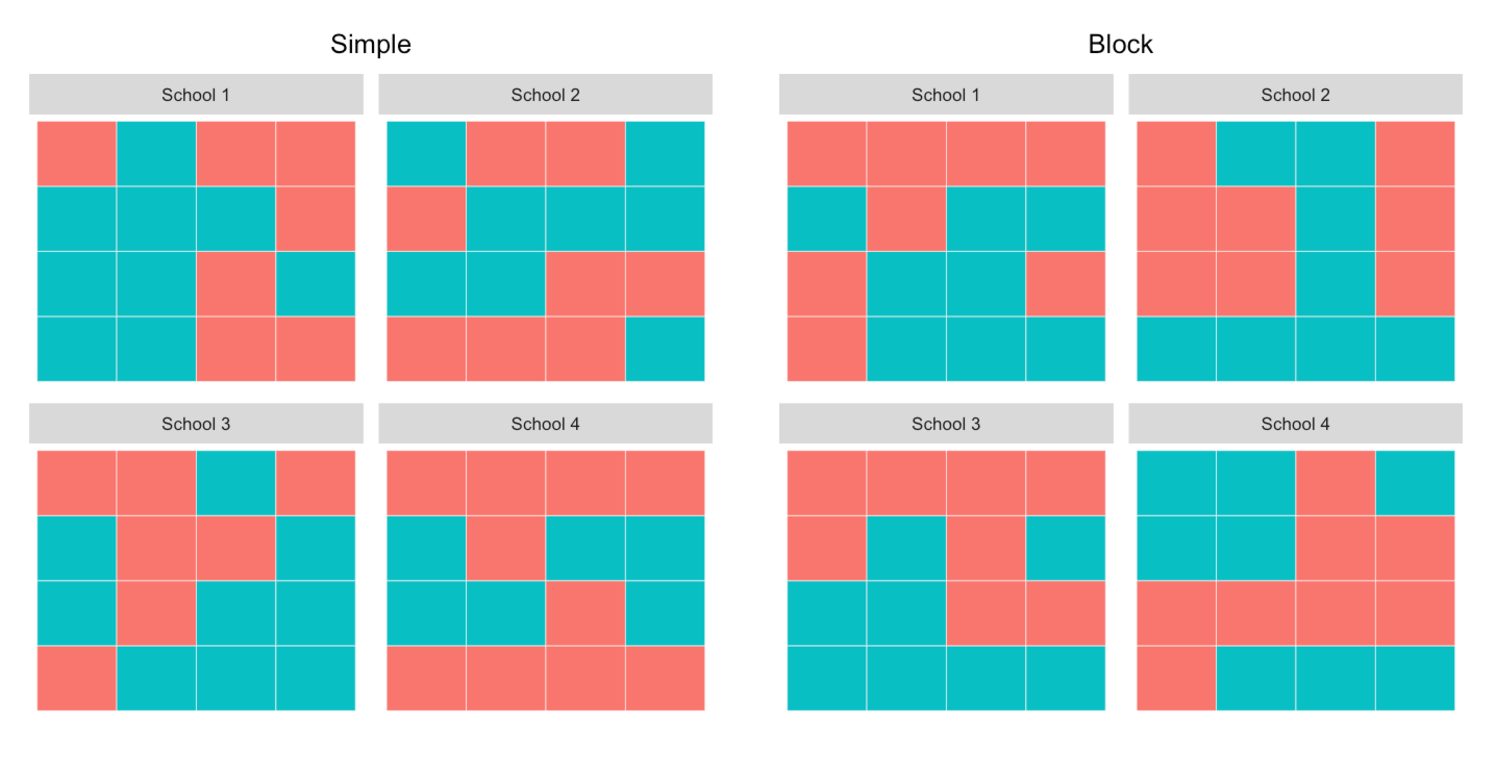
\includegraphics{figs/blocking}
\end{frame}

\end{document}
